\section{Calculus and Polar Functions} \label{sec:polarcalc}
The previous section defined polar coordinates, leading to polar functions. We investigated plotting these functions and solving a fundamental question about their graphs, namely, where do two polar graphs intersect?

We now turn our attention to answering other questions, whose solutions require the use of calculus. A basis for much of what is done in this section is the ability to turn a polar function $r=f(\theta)$ into a set of parametric equations. Using the identities $x=r\cos \theta$ and $y=r\sin \theta$, we can create the parametric equations $x=f(\theta)\cos\theta$, $y=f(\theta)\sin\theta$ and apply the concepts of Section \ref{sec:par_calc}.\\

\noindent\textbf{\large Polar Functions and $\ds \frac{dy}{dx}$}\\

We are interested in the lines tangent a given graph, regardless of whether that graph is produced by rectangular, parametric, or polar equations. In each of these contexts, the slope of the tangent line is $\frac{dy}{dx}$. Given $r=f(\theta)$, we are generally \textit{not} concerned with $r\,'=\fp(\theta)$; that describes how fast $r$ changes with respect to $\theta$. Instead, we will use $x=f(\theta)\cos\theta$, $y=f(\theta)\sin\theta$ to compute $\frac{dy}{dx}$. 

Using Key Idea \ref{idea:dydxpar} we have $$\frac{dy}{dx} = \frac{dy}{d\theta}\Big/\frac{dx}{d\theta}.$$ Each of the two derivatives on the right hand side of the equality requires the use of the Product Rule. We state the important result as a Key Idea.\\

\keyidea{idea:dydxpol}{Finding $\frac{dy}{dx}$ with Polar Functions}
{Let $r=f(\theta)$ be a polar function. With $x=f(\theta)\cos\theta$ and $y=f(\theta)\sin\theta$,
\index{polar!functions!finding $\frac{dy}{dx}$}\index{tangent line}
$$\frac{dy}{dx} = \frac{\fp(\theta)\sin\theta+f(\theta)\cos\theta}{\fp(\theta)\cos\theta-f(\theta)\sin\theta}.$$
}

\example{ex_polcalc1}{Finding $\frac{dy}{dx}$ with polar functions.}
{Consider the lima\c con $r=1+2\sin\theta$ on $[0,2\pi]$.
\begin{enumerate}
	\item Find the equations of the tangent and normal lines to the graph at $\theta=\pi/4$.
	\item		Find where the graph has vertical and horizontal tangent lines.
\end{enumerate}
}
{\begin{enumerate}
	\item We start by computing $\frac{dy}{dx}$. With $\fp(\theta) = 2\cos\theta$, we have
	\begin{align*}
	\frac{dy}{dx} &= \frac{2\cos\theta\sin\theta + \cos\theta(1+2\sin\theta)}{2\cos^2\theta-\sin\theta(1+2\sin\theta)}\\
	&= \frac{\cos\theta(4\sin\theta+1)}{2(\cos^2\theta-\sin^2\theta)-\sin\theta}.
	\end{align*}
	When $\theta=\pi/4$, $\frac{dy}{dx}=-2\sqrt{2}-1$ (this requires a bit of simplification). In rectangular coordinates, the point on the graph at $\theta=\pi/4$ is $(1+\sqrt{2}/2,1+\sqrt{2}/2)$. Thus the rectangular equation of the line tangent to the lima\c con at $\theta=\pi/4$ is 
	$$y=(-2\sqrt{2}-1)\big(x-(1+\sqrt{2}/2)\big)+1+\sqrt{2}/2 \approx  -3.83 x+8.24.$$ The lima\c con and the tangent line are graphed in Figure \ref{fig:polcalc1}. 
	
	The normal line has the opposite--reciprocal slope as the tangent line, so its equation is 
	$$y \approx \frac{1}{3.83}x+1.26.$$
	\mfigure{.75}{The lima\c con in Example \ref{ex_polcalc1} with its tangent line at $\theta=\pi/4$ and points of vertical and horizontal tangency.}{fig:polcalc1}{figures/figpolcalc1}
	\drawexampleline
	
	\item		To find the horizontal lines of tangency, we find where $\frac{dy}{dx}=0$; thus we find where the numerator of our equation for $\frac{dy}{dx}$ is 0.
	$$\cos\theta(4\sin\theta+1)=0\quad \Rightarrow \quad \cos\theta=0 \quad \text{or}\quad 4\sin\theta+1=0.$$
	On $[0,2\pi]$, $\cos\theta=0$ when $\theta=\pi/2,\ 3\pi/2$. 

Setting $4\sin\theta+1=0$ gives $\theta=\sin^{-1}(-1/4)\approx -0.2527 = -14.48^\circ$. We want the results in $[0,2\pi]$; we also recognize there are two solutions, one in the 3$^\text{rd}$ quadrant and one in the 4$^\text{th}$. Using reference angles, we have our two solutions as $\theta =3.39$ and $6.03$ radians. The four points we obtained where the lima\c con has a horizontal tangent line are given in Figure \ref{fig:polcalc1} with black--filled dots.\\

To find the vertical lines of tangency, we set the denominator of $\frac{dy}{dx}=0$. 
\begin{align*}
2(\cos^2\theta -\sin^2\theta)-\sin\theta &= 0 .
\intertext{Convert the $\cos^2\theta$ term to $1-\sin^2\theta$:}
2(1-\sin^2\theta-\sin^2\theta)-\sin\theta &= 0\\
4\sin^2\theta + \sin\theta -2 &= 0.
\intertext{Recognize this as a quadratic in the variable $\sin\theta$. Using the quadratic formula, we have}
\sin\theta &= \frac{-1\pm\sqrt{33}}{8}.
\end{align*}
We solve $\sin\theta = \frac{-1+\sqrt{33}}8$ and $\sin\theta = \frac{-1-\sqrt{33}}8$:
\begin{align*}
\sin\theta &=\frac{-1+\sqrt{33}}8 & \sin\theta &= \frac{-1-\sqrt{33}}{8}\\
\theta &= \sin^{-1}\left(\frac{-1+\sqrt{33}}8\right) & \theta &= \sin^{-1}\left(\frac{-1-\sqrt{33}}8\right)\\
\theta &= 0.6349 & \theta &= -1.0030
\end{align*}
In each of the solutions above, we only get one of the possible two solutions as $\sin^{-1}x$ only returns solutions in $[-\pi/2,\pi/2]$, the 4$^\text{th}$ and $1^\text{st}$ quadrants. Again using reference angles, we have:
$$\sin\theta = \frac{-1+\sqrt{33}}8 \quad \Rightarrow \quad \theta = 0.6349,\ 2.5067 \text{ radians}$$
and 
$$\sin\theta = \frac{-1-\sqrt{33}}8 \quad \Rightarrow \quad \theta = 4.1446,\ 5.2802 \text{ radians.}$$
These points are also shown in Figure \ref{fig:polcalc1} with white--filled dots.
	\end{enumerate}
	\vskip-\baselineskip
}\\

When the graph of the polar function $r=f(\theta)$ intersects the pole, it means that $f(\alpha)=0$ for some angle $\alpha$. Thus the formula for $\frac{dy}{dx}$ in such instances is very simple, reducing simply to $$\frac{dy}{dx} = \tan \alpha.$$
This equation makes an interesting point. It tells us the slope of the tangent line at the pole is $\tan \alpha$; some of our previous work (see, for instance, Example \ref{ex_polar3}) shows us that the line through the pole with slope $\tan \alpha$ has polar equation $\theta=\alpha$. Thus when a polar graph touches the pole at $\theta=\alpha$, the equation of the tangent line at the pole is $\theta=\alpha$. \\

\example{ex_polcalc2}{Finding tangent lines at the pole.}{
Let $r=1+2\sin\theta$, a lima\c con. Find the equations of the lines tangent to the graph at the pole.
\mfigure{.35}{Graphing the tangent lines at the pole in Example \ref{ex_polcalc2}.}{fig:polcalc2}{figures/figpolcalc2}}
{We need to know when $r=0$. 
\begin{align*}
1+2\sin\theta &= 0\\
\sin\theta &= -1/2\\
\theta &= \frac{7\pi}{6},\ \frac{11\pi}6.
\end{align*}
Thus the equations of the tangent lines, in polar, are $\theta = 7\pi/6$ and $\theta = 11\pi/6$. In rectangular form, the tangent lines are $y=\tan(7\pi/6)x$ and $y=\tan(11\pi/6)x$. The full lima\c con can be seen in Figure \ref{fig:polcalc1}; we zoom in on the tangent lines in Figure \ref{fig:polcalc2}.
}\\

\noindent\textbf{\large Area}\\

When using rectangular coordinates, the equations $x=h$ and $y=k$ defined vertical and horzontal lines, respectively, and combinations of these lines create rectangles (hence the name ``rectangular coordinates''). It is then somewhat natural to use rectangles to approximate area as we did when learning about the definite integral.\index{polar!functions!area}

When using polar coordinates, the equations $\theta=\alpha$ and $r=c$ form lines through the origin and circles centered at the origin, respectively, and combinations of these curves form sectors of circles. It is then somewhat natural to calculate the area of regions defined by polar functions by first approximating with sectors of circles. 

Consider Figure \ref{fig:polararea} (a) where a region defined by $r=f(\theta)$ on $[\alpha,\beta]$ is given. (Note how the ``sides'' of the region are the lines $\theta=\alpha$ and $\theta=\beta$, whereas in rectangular coordinates the ``sides'' of regions were often the vertical lines $x=a$ and $x=b$.)
\mnote{.8}{\textbf{Note:} Recall that the area of a sector of a circle with radius $r$ subtended by an angle $\theta$ is $A = \frac12\theta r^2$.

\hfill
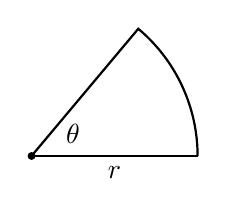
\begin{tikzpicture}[x=30pt,y=30pt,thick]
			\draw (2,0) arc (0:50:2) -- (0,0);
			\draw [] (0,0) -- (2,0) node [pos=.5,below] {$r$};
			\draw [fill=black] (0,0) circle (1pt);
			%\draw (1.95,1.0) node {$s$};
			\draw (0,0) node [shift={(15pt,8pt)}] {$\theta$};
			\end{tikzpicture}
\hfill\null
}

Partition the interval $[\alpha,\beta]$ into $n$ equally spaced subintervals as $\alpha = \theta_1 < \theta_2 <\cdots <\theta_{n+1}=\beta$. The length of each subinterval is $\Delta\theta = (\beta-\alpha)/n$, representing a small change in angle. The area of the region defined by the $i\,^\text{th}$ subinterval $[\theta_i,\theta_{i+1}]$ can be approximated with a sector of a circle with radius $f(c_i)$, for some $c_i$ in $[\theta_i,\theta_{i+1}]$. The area of this sector is $\frac12f(c_i)^2\Delta\theta$. This is shown in part (b) of the figure, where $[\alpha,\beta]$ has been divided into 4 subintervals. We approximate the area of the whole region by summing the areas of all sectors:
$$\text{Area} \approx \sum_{i=1}^n \frac12f(c_i)^2\Delta\theta.$$
This is a Riemann sum. By taking the limit of the sum as $n\to\infty$, we find the exact area of the region in the form of a definite integral.
\mtable{.5}{Computing the area of a polar region.}{fig:polararea}{%
\begin{tabular}{c}
\myincludegraphics{figures/figpolarea1}\\
(a)\\[10pt]
\myincludegraphics{figures/figpolarea2}\\
(b)
\end{tabular}
}
\enlargethispage{2\baselineskip}
%\clearpage

\theorem{thm:polar_area}{Area of a Polar Region}
{Let $f$ be continuous and non-negative on $[\alpha,\beta]$, where $0\leq \beta-\alpha\leq 2\pi$. The area  $A$ of the region bounded by the curve $r=f(\theta)$ and the lines $\theta=\alpha$ and $\theta=\beta$ is 
$$
A \ =\  \frac12\int_\alpha^\beta f(\theta)^2 \ d\theta\  =\  \frac12\int_\alpha^\beta r^{\,2} \ d\theta$$
}

The theorem states that $0\leq \beta-\alpha\leq 2\pi$. This ensures that region does not overlap itself, which would give a result that does not correspond directly to the area.\\

\example{ex_polcalc3}{Area of a polar region}{
Find the area of the circle defined by $r=\cos \theta$. (Recall this circle has radius $1/2$.)}
{This is a direct application of Theorem \ref{thm:polar_area}. The circle is traced out on $[0,\pi]$, leading to the integral
\begin{align*}
\text{Area} &= \frac12\int_0^\pi \cos^2\theta\ d  \theta \\
						&= \frac12\int_0^\pi \frac{1+\cos(2\theta)}{2}\ d\theta\\
						&= \frac14\big(\theta +\frac12\sin(2\theta)\big)\Bigg|_0^\pi\\
						&= \frac14\pi.
\end{align*}
Of course, we already knew the area of a circle with radius $1/2$. We did this example to demonstrate that the area formula is correct.
}\\

\mnote{.7}{\textbf{Note:} Example \ref{ex_polcalc3} requires the use of the integral $\ds\int \cos^2\theta\ d\theta$. This is handled well by using the power reducing formula as found in the back of this text. Due to the nature of the area formula, integrating $\cos^2\theta$ and $\sin^2\theta$ is required often. We offer here these indefinite integrals as a time--saving measure.\\
$$\int\cos^2\theta\ d\theta = \frac12\theta+\frac14\sin(2\theta)+C$$
$$\int\sin^2\theta\ d\theta = \frac12\theta-\frac14\sin(2\theta)+C$$
}

\example{ex_polcalc4}{Area of a polar region}{
Find the area of the cardiod $r=1+\cos\theta$ bound between $\theta=\pi/6$ and $\theta=\pi/3$, as shown in Figure \ref{fig:polcalc4}.
\mfigure{.3}{Finding the area of the shaded region of a cardiod in Example \ref{ex_polcalc4}.}{fig:polcalc4}{figures/figpolcalc4}
}
{This is again a direct application of Theorem \ref{thm:polar_area}. 
\begin{align*}
\text{Area} &= \frac12\int_{\pi/6}^{\pi/3} (1+\cos\theta)^2\ d\theta\\
				&= \frac12\int_{\pi/6}^{\pi/3} (1+2\cos\theta+\cos^2\theta)\ d\theta\\
				&= \frac12\left(\theta+2\sin\theta+\frac12\theta+\frac14\sin(2\theta)\right)\Bigg|_{\pi/6}^{\pi/3} \\
				&= \frac18\big(\pi+4\sqrt{3}-4\big) \approx 0.7587.
				\end{align*}
\vskip-\baselineskip
}\\

\noindent\textbf{Area Between Curves}\\

Our study of area in the context of rectangular functions led naturally to finding area bounded between curves. We consider the same in the context of polar functions. \index{polar!functions!area between curves}

Consider the shaded region shown in Figure \ref{fig:polarea3}. We can find the area of this region by computing the area bounded by $r_2=f_2(\theta)$ and subtracting the area bounded by $r_1=f_1(\theta)$ on $[\alpha,\beta]$. Thus
$$\text{Area}\ = \ \frac12\int_\alpha^\beta r_2^{\,2}\ d\theta - \frac12\int_\alpha^\beta r_1^{\,2}\ d\theta = \frac12\int_\alpha^\beta \big(r_2^{\,2}-r_1^{\,2}\big)\ d\theta.$$
\mfigure{.6}{Illustrating area bound between two polar curves.}{fig:polarea3}{figures/figpolarea3}

\keyidea{idea:area_between_polar}{Area Between Polar Curves}
{The area $A$ of the region bounded by $r_1=f_1(\theta)$ and $r_2=f_2(\theta)$, $\theta=\alpha$ and $\theta=\beta$, where $f_1(\theta)\leq f_2(\theta)$ on $[\alpha,\beta]$, is
$$A = \frac12\int_\alpha^\beta \big(r_2^{\,2}-r_1^{\,2}\big)\ d\theta.$$
}

\enlargethispage{2\baselineskip}
\example{ex_polcalc5}{Area between polar curves}{
Find the area bounded between the curves $r=1+\cos \theta$ and $r=3\cos\theta$, as shown in Figure \ref{fig:polcalc5}.
\mfigure{.3}{Finding the area between polar curves in Example \ref{ex_polcalc5}.}{fig:polcalc5}{figures/figpolcalc5}
}
{We need to find the points of intersection between these two functions. Setting them equal to each other, we find:
\begin{align*}
1+\cos\theta &= 3\cos \theta \\
 \cos\theta &=1/2\\
\theta &= \pm \pi/3
\end{align*}
Thus we integrate $\frac12\big((3\cos\theta)^2-(1+\cos\theta)^2\big)$ on $[-\pi/3,\pi/3]$.
\begin{align*}
\text{Area} &= \frac12\int_{-\pi/3}^{\pi/3} \big((3\cos\theta)^2-(1+\cos\theta)^2\big)\ d\theta\\
		&= \frac12\int_{-\pi/3}^{\pi/3} \big( 8\cos^2\theta-2\cos\theta-1\big)\ d\theta \\
		&= \frac12\big(2\sin(2\theta) - 2\sin\theta+3\theta\big)\Bigg|_{-\pi/3}^{\pi/3}\\
		&= \pi.
\end{align*}
Amazingly enough, the area between these curves has a ``nice'' value.
}\\

\example{ex_polcalc6}{Area defined by polar curves}{
Find the area bounded between the polar curves $r=1$ and $r=2\cos(2\theta)$, as shown in Figure \ref{fig:polcalc6} (a).}
{We need to find the point of intersection between the two curves. Setting the two functions equal to each other, we have
$$2\cos(2\theta) = 1 \quad \Rightarrow \quad \cos(2\theta) = \frac12 \quad \Rightarrow \quad 2\theta = \pi/3\quad \Rightarrow \quad \theta=\pi/6.$$
\mtable{.4}{Graphing the region bounded by the functions in Example \ref{ex_polcalc6}.}{fig:polcalc6}{%
\begin{tabular}{c}
\myincludegraphics{figures/figpolcalc6}\\
(a)\\[10pt]
\myincludegraphics{figures/figpolcalc6a}\\
(b)\\
\end{tabular}
}
In part (b) of the figure, we zoom in on the region and note that it is not really bounded \textit{between} two polar curves, but rather \textit{by} two polar curves, along with $\theta=0$. The dashed line breaks the region into its component parts. Below the dashed line, the region is defined by $r=1$, $\theta=0$ and $\theta = \pi/6$. (Note: the dashed line lies on the line $\theta=\pi/6$.) Above the dashed line the region is bounded by $r=2\cos(2\theta)$ and $\theta =\pi/6$. Since we have two separate regions, we find the area using two separate integrals.

Call the area below the dashed line $A_1$ and the area above the dashed line $A_2$. They are determined by the following integrals:
$$A_1 = \frac12\int_0^{\pi/6} (1)^2\ d\theta\qquad  A_2 = \frac12\int_{\pi/6}^{\pi/4} \big(2\cos(2\theta)\big)^2\ d\theta.$$
(The upper bound of the integral computing $A_2$ is $\pi/4$ as $r=2\cos(2\theta)$ is at the pole when $\theta=\pi/4$.)

We omit the integration details and let the reader verify that $A_1 = \pi/12$ and $A_2 = \pi/12-\sqrt{3}/8$; the total area is $A = \pi/6-\sqrt{3}/8$.
}\\

\noindent\textbf{\large Arc Length}\\

As we have already considered the arc length of curves defined by rectangular and parametric equations, we now consider it in the context of polar equations. Recall that the arc length $L$ of the graph defined by the parametric equations $x=f(t)$, $y=g(t)$ on $[a,b]$ is
\index{arc length}\index{polar!function!arc length}
\begin{equation}L = \int_a^b \sqrt{\fp(t)^2 + g\primeskip'(t)^2}\ dt = \int_a^b \sqrt{x\primeskip'(t)^2+y\primeskip'(t)^2}\ dt.\label{eq:polar_arclength}\end{equation}

Now consider the polar function $r=f(\theta)$. We again use the identities $x=f(\theta)\cos\theta$ and $y=f(\theta)\sin\theta$ to create parametric equations based on the polar function. We compute $x\primeskip'(\theta)$ and $y\primeskip'(\theta)$ as done before when computing $\frac{dy}{dx}$, then apply Equation \eqref{eq:polar_arclength}.

The expression $x\primeskip'(\theta)^2+y\primeskip'(\theta)^2$ can be simplified a great deal; we leave this as an exercise and state that $$x\primeskip'(\theta)^2+y\primeskip'(\theta)^2 = \fp(\theta)^2+f(\theta)^2.$$ This leads us to the  arc length formula.

\keyidea{idea:polar_arclength}{Arc Length of Polar Curves}
{Let  $r=f(\theta)$ be a polar function with $\fp$ continuous on an open interval $I$ containing $[\alpha,\beta]$, on which the graph traces itself only once. The arc length $L$ of the graph on $[\alpha,\beta]$ is
$$L = \int_\alpha^\beta \sqrt{\fp(\theta)^2+f(\theta)^2}\ d\theta = \int_\alpha^\beta\sqrt{(r\,')^2+ r^2}\ d\theta.$$
}

\example{ex_polcalc7}{Arc length of a lima\c con}{
Find the arc length of the lima\c con $r=1+2\sin t$.}
{With $r=1+2\sin t$, we have $r\,' = 2\cos t$. The lima\c con is traced out once on $[0,2\pi]$, giving us our bounds of integration. Applying Key Idea \ref{idea:polar_arclength}, we have
\begin{align*}
L 	&= \int_0^{2\pi} \sqrt{(2\cos\theta)^2+(1+2\sin\theta)^2}\ d\theta \\
		&=	\int_0^{2\pi} \sqrt{4\cos^2\theta+4\sin^2\theta +4\sin\theta+1}\ d\theta\\
		&=	\int_0^{2\pi} \sqrt{4\sin\theta+5}\ d\theta\\
		&\approx 13.3649.
\end{align*}
\mfigure{.8}{The lima\c con in Example \ref{ex_polcalc7} whose arc length is measured.}{fig:polcalc7}{figures/figpolcalc7}
The final integral cannot be solved in terms of elementary functions, so we resorted to a numerical approximation. (Simpson's Rule, with $n=4$, approximates the value with $13.0608$. Using $n=22$ gives the value above, which is accurate to 4 places after the decimal.) 
}\\

\noindent\textbf{\large Surface Area}\\

The formula for arc length leads us to a formula for surface area. The following Key Idea is based on Key Idea \ref{idea:surface_area_parametric}.

\keyidea{idea:surface_area_polar}{Surface Area of a Solid of Revolution}
{Consider the graph of the polar equation $r=f(\theta)$, where $\fp$ is continuous on an open interval containing $[\alpha,\beta]$ on which the graph does not cross itself.
\index{surface area!solid of revolution}\index{polar!function!surface area}\index{integration!surface area}
	\begin{enumerate}
		\item The surface area of the solid formed by revolving the graph about the initial ray ($\theta=0$) is:
		$$\text{Surface Area} = 2\pi\int_\alpha^\beta f(\theta)\sin\theta\sqrt{\fp(\theta)^2+f(\theta)^2}\ d\theta.$$
		\item The surface area of the solid formed by revolving the graph about the line $\theta=\pi/2$ is:
		$$\text{Surface Area} = 2\pi\int_\alpha^\beta f(\theta)\cos\theta\sqrt{\fp(\theta)^2+f(\theta)^2}\ d\theta.$$
	\end{enumerate}
}
\clearpage

\example{ex_polcalc8}{Surface area determined by a polar curve}{
Find the surface area formed by revolving one petal of the rose curve $r=\cos(2\theta)$ about its central axis (see Figure \ref{fig:polcalc8}).}
{\mtable{.7}{Finding the surface area of a rose--curve petal that is revolved around its central axis.}{fig:polcalc8}{%
\begin{tabular}{c}
\myincludegraphics{figures/figpolcalc8}\\
(a)\\[10pt]
%%\ifthenelse{\boolean{in_threeD}}{{%
%%\myincludegraphicsthree[width=150pt,3Dmenu,activate=onclick,deactivate=pageinvisible,
%%3Droll=0,
%%3Dortho=0.009,
%%3Dc2c=0.41893383860588074 -0.887881875038147 0.1901581883430481,
%%3Dcoo=65.85308837890625 6.341495513916016 17.98039436340332,
%%3Droo=85,
%%3Dlights=Headlamp,add3Djscript=asylabels.js]{figures/figpolcalc8a_3D}}}%
%%{\myincludegraphics[scale=1.25,trim=5mm 5mm 5mm 5mm,clip=true]{figures/figpolcalc8a}}\\
%%%\myincludegraphicsthree{width=150pt,3Dmenu,activate=onclick,deactivate=pageinvisible,
%%%3Droll=0,
%%%3Dortho=0.009,
%%%3Dc2c=0.41893383860588074 -0.887881875038147 0.1901581883430481,
%%%3Dcoo=65.85308837890625 6.341495513916016 17.98039436340332,
%%%3Droo=85,
%%%3Dlights=Headlamp,add3Djscript=asylabels.js}{scale=1.25,trim=5mm 5mm 5mm 5mm,clip=true}{figures/figpolcalc8a}\\
%%\myincludegraphics[scale=1.25,trim=5mm 5mm 5mm 5mm,clip=true]{figures/figpolcalc8a}\\
\myincludegraphicsthree{width=150pt,3Dmenu,activate=onclick,deactivate=pageinvisible,
3Droll=0,
3Dortho=0.009,
3Dc2c=0.41893383860588074 -0.887881875038147 0.1901581883430481,
3Dcoo=65.85308837890625 6.341495513916016 17.98039436340332,
3Droo=85,
3Dlights=Headlamp,add3Djscript=asylabels.js}{scale=1.25,trim=5mm 5mm 5mm 5mm,clip=true}{figures/figpolcalc8a}\\
(b)\\
\end{tabular}
}
We choose, as implied by the figure, to revolve the portion of the curve that lies on $[0,\pi/4]$ about the initial ray. Using Key Idea \ref{idea:surface_area_polar} and the fact that $\fp(\theta) = -2\sin(2\theta)$, we have
\begin{align*}
\text{Surface Area} &= 2\pi\int_0^{\pi/4} \cos(2\theta)\sin(\theta)\sqrt{\big(-2\sin(2\theta)\big)^2+\big(\cos(2\theta)\big)^2}\ d\theta \\
&\approx 1.36707.
\end{align*}
The integral is another that cannot be evaluated in terms of elementary functions. Simpson's Rule, with $n=4$, approximates the value at $1.36751$.%; with $n=10$, the value is accurate to 4 decimal places.
}\\


This chapter has been about curves in the plane. While there is great mathematics to be discovered in the two dimensions of a plane, we live in a three dimensional world and hence we should also look to do mathematics in 3D -- that is, in \emph{space}. The next chapter begins our exploration into space by introducing the topic of \emph{vectors}, which are incredibly useful and powerful mathematical objects.
\printexercises{exercises/09_05_exercises}